\chapter{Implementation}
\section{Methodology}

As a reminder of the objective, there are camera traps that produce images and videos, ecologists want to have statistics on species to prevent their extinction.
At the moment, they recognize and count species manually, spending hours watching videos and photos, it takes a lot of time and is therefore very expensive.

The solution is to automatize this process with computer vision, this must meet the "four easy constraints":
\begin{itemize}
    \item Easy to deploy because ecologist usually don't have much computer science knowledge.
    \item Easy to maintain because we don't want something that need 10 hours/day monitoring if anything went wrong.
    \item Easy to scale, being able to handle either 1000 images / month or 1 000 000 images / month.
    \item Easy to price, having a fully transparent estimation of the different costs.
\end{itemize}

\pagebreak\subsection{Existing solutions}
\subsubsection{Microsoft Camera trap}
Microsoft AI for Earth propose a set of tools and algorithms especially designed for camera traps monitoring\cite{microsoft_camera_trap}.

It goes from data parsing scripts, pre-trained models on camera-trap images or web interfaces to use their models ...

An example of the model has been developed (see Figure ~\ref{fig:microsoftcamtrap}).

\begin{figure}[H]
\centering
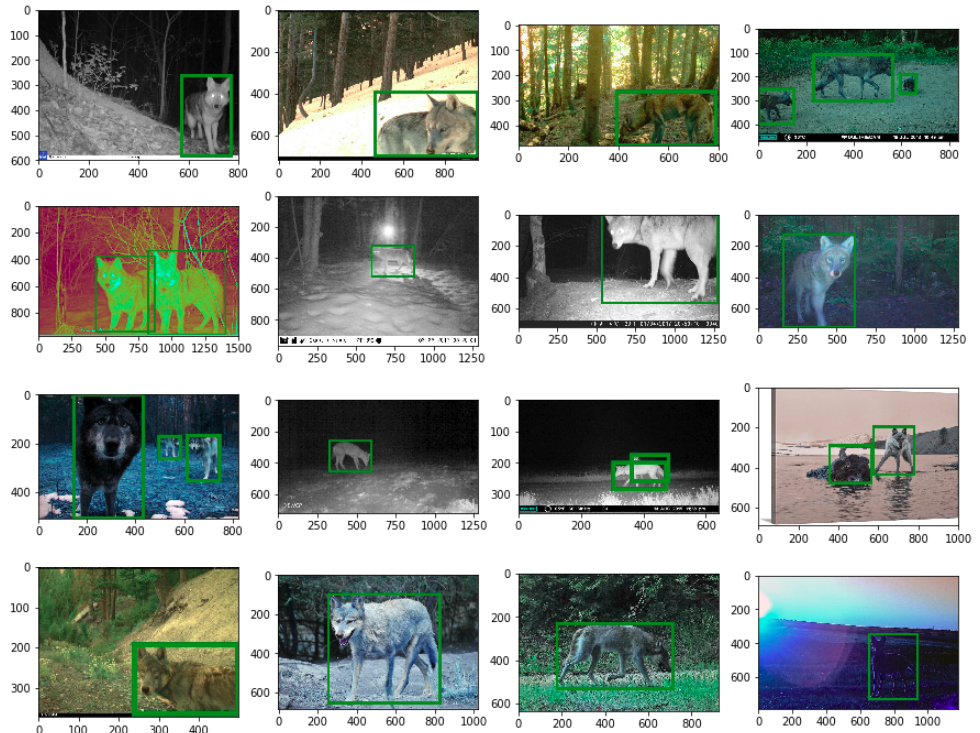
\includegraphics[width=.7\linewidth]{wolves_detected.png}
\caption{Example usage of Microsoft's camera trap model. \href{https://gist.github.com/louis030195/b64ba5a839c46c2ab0bf9451477a97df}{Source}}
\label{fig:microsoftcamtrap}
\end{figure}

This solution is not usable in production, it is a bit messy and no clear direction is given.
\subsubsection{Google DeepMind camera trap}
DeepMind, one of the lead actor in artificial intelligence research, the author of the major breakthroughs in AI, such as AlphaGo\cite{alphago}, AlphaStar\cite{alphastar} and much more are begining to take an interest in accelerate ecological research using machine learning\cite{deepmind_camera_trap}.
Their recent announcement is nevertheless rather vague, just an article and no code is available, they seems to work on training algorithm on the Seregenti Snapshot datasets.

Their solution will probably be interesting but not available in the short term

\subsection{Considered solutions}
Running a dedicated server is hard to deploy, it requires the implementation of containers, container-orchestration pipelines and other infrastructure tools.
To maintain it properly you also need to develop additional monitoring tools in order to keep track of its state.
It is also difficult to scale due to the work required on hardware side and finally the price can still be high.

With cloud providers (Amazon, Google, Microsoft, DigitalOcean ...) no need to worry about infrastructure, hardware, easy to deploy, maintain, scale and relatively price transparent.

We use Google Cloud Platform as a choice of experience, long-term potential and machine learning and big data orientation.


\pagebreak\section{Technologies}
\subsection{Machine learning}
Python has been chosen because it is the most popular programming language for machine learning\cite{python_machine_learning} due to numerous advantages:
\begin{itemize}
    \item Machine learning, vectors, math, visualisation libraries
    \item Massive community
    \item Machine learning frameworks
    \item Fast results
\end{itemize}

Next, usually the choice of framework have to been done between the most popular: Google's Tensorflow\cite{tensorflow} or Facebook's Pytorch\cite{pytorch}.

Both are open-source, the most important difference between the two is the way these frameworks define the computational graphs. While Tensorflow creates a static graph, PyTorch believes in a dynamic graph.
It means that Tensorflow is more difficult to learn at the moment, but Tensorflow will soon be released as 2.0 and it will be possible to create dynamic graph like Pytorch.
Tensorflow has way bigger community, more tools (Tensorboard, Tensorflow-serving ...).
Also it is obviously easier to use Google services with Tensorflow than Pytorch, for all these reasons Tensorflow has been chosen.

\pagebreak\subsection{Google Cloud Platform}
Google Cloud Platform is the platform that brings together Google's various cloud services. 
The Google Cloud Platform is a suite of cloud services offered by Google. The platform includes various cloud services for computing, storage, networking, Big Data, machine learning, Internet of things, security, cloud management and application development that are directly launched on Google's servers.

\subsubsection{Advantages}

Like all cloud platforms, Google's platform has the advantage of sparing companies the management of an infrastructure, server provisioning and network configuration. In addition, Google also highlights the evolutionary aspect of its infrastructure. Constantly updated and optimized, the platform benefits from Google's expertise and is efficient, economical and secure.

With the fully managed, server-less computing system, users can move from prototype to global production without worrying about capacity, reliability or performance. Other strengths of the Google Cloud Platform include a data center backbone network composed of thousands of kilometers of fiber optic cables combined with an advanced networking solution and edge caching services to deliver extreme performance.

\subsubsection{Services}

\begin{figure}[H]
    \centering
    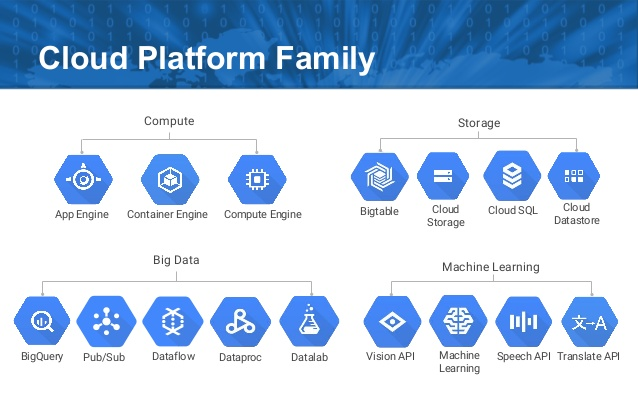
\includegraphics[scale = 0.55]{google-cloud-platform-services.jpg}
	\caption{Google Cloud Platform services}
	\label{fig:gcp}
\end{figure}


The Google Compute Engine is an Infrastructure as a Service (IaaS) that allows users to launch instances of virtual machines. This allows them to run their workloads on the cloud (see Figure ~\ref{fig:gcp}).

\begin{itemize}
    \item The Google App Engine is a Platform as a Service (PaaS). It allows software developers to access a scalable hosting offer. Developers can use an SDK to develop software that is compatible with the App Engine.
    \item Google Cloud Storage is a cloud storage platform designed to store large unstructured data sets. Google also offers database storage options, such as the Datastore for NoSQL storage, or CloudSQL for MySQL. We also find the native database Bigtable.
    \item The Google Container Engine is a management and orchestration system for Docker containers running on Google's public cloud. This system is based on the Google Kubernetes container orchestration engine.
The Google Cloud Platform also offers application development and integration services. For example, Cloud Pub/Sub is a real-time messaging service that allows messages to be exchanged between applications. Similarly, Endpoints allows developers to create services based on RESTful APIs and make these services very accessible.
\end{itemize}


\subsubsection{Other services}

Google also offers higher-level services on its Cloud platform, such as those dedicated to Big Data and Machine Learning. Google's Big Data services are used to process and analyze data. Google BigQuery allows you to search for data sets of several terabytes, for example. Dataflow is a data processing service designed for data analysis, extraction, transformation and loading. Dataproc offers Apache Spark and Hadoop services for Big Data processing. It also integrates the databases of Cassandra and MongoDB.

In terms of artificial intelligence, Google offers its Cloud Machine Learning Engine(Google Cloud AI Platform), a managed service that allows users to develop and train Machine Learning models. Different APIs are also available for the translation and analysis of speech, text, images or videos.
AI Platform allow to deploy any model in the Tensorflow SavedModel format, while the different API such as Video Intelligence is simple to use but is, at the moment, only for general use cases, for example it won't we suitable for camera-trap images.

\subsubsection{Prices}

Like most cloud service providers, Google Cloud Platform pricing is based on a pay-as-you-go (pay-per-use) business model, which means that users pay according to the resources they consume. Resource consumption is accurately calculated to the minute. According to Google, the platform's rates are on average 60\% lower than those of other providers\cite{gcp_pricing}.

The other advantage of this model is that users do not have to pay upfront fees. Similarly, billing ends as soon as the user ceases to use the services without having to pay termination fees. For Google Compute Engine and Cloud SQL services, Google also offers an automatic discount system of up to 30\% on the most used workloads. Rates vary between the different services and should therefore be consulted on a case-by-case basis on the official website.

\pagebreak\subsection{Front end}
We have chosen to use Javascript, which is the most popular language for the front end.
Front end web development is a field that is evolving very quickly and solutions are quickly becoming obsolete.

Especially, we use Lit-Element which is created to support a component-oriented approach to front-end Web development.

Lit-Element is an open-source JavaScript library used to develop Web applications using Web components. Created by Google developers and contributors on GitHub.

The advantage of Lit-Element is that you don't need to know in detail how it works unlike popular front end heavy frameworks such as Angular, React, Vue and others.

\pagebreak\section{Online versus Batch predictions}
AI Platform offers two methods for obtaining predictions from trained models: online prediction and batch prediction. In both cases, you transmit input data to a machine learning model hosted in the cloud and obtain inferences for each instance of data (see the differences in Figure ~\ref{fig:onlinebatch}).

\begin{figure}[H]
    \centering
    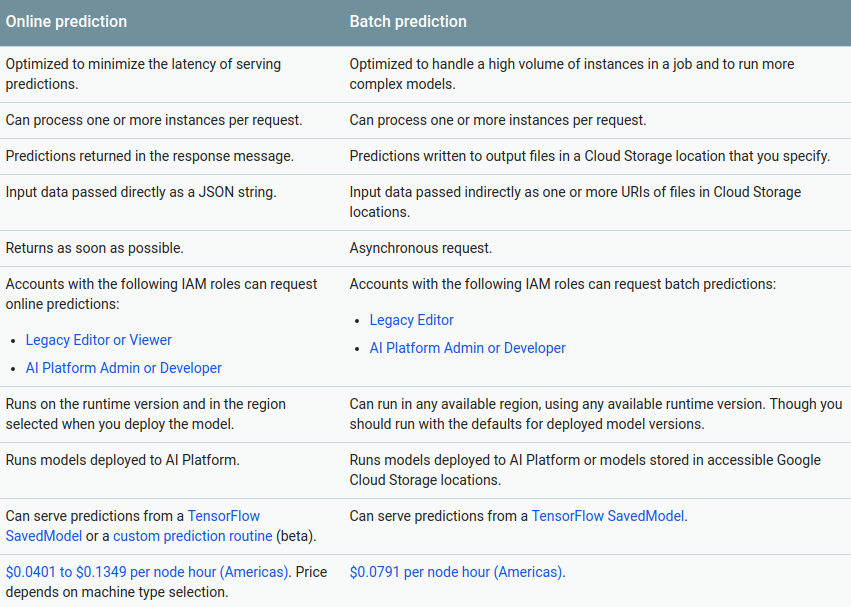
\includegraphics[scale = 0.5]{online_vs_batch.png}
	\caption{Online versus batch predictions. \href{https://cloud.google.com/ml-engine/docs/tensorflow/online-vs-batch-prediction}{Source}}
	\label{fig:onlinebatch}
\end{figure}

It is generally preferable to use online prediction to make requests in response to an application entry or in other situations where rapid inference is required.

Batch prediction is ideal when processing accumulated data, when you do not need immediate results. For example, a periodic task that makes predictions from all the data collected since the last task.

You must also make your decision taking into account potential variations in the cost of prediction.

Here we obviously chose batch prediction because our goal is to have statistics of species over long times, we don't need to have instant result, the user will drop big amount of videos / photos that will be processed.

\subsubsection{Latency of batch prediction}
If you use a simple model and a small set of input instances, you will find that, to complete identical prediction requests, there is a considerable difference in the time required if online prediction is used compared to batch prediction. A batch task can take several minutes to complete predictions that would be returned almost instantly by an online request. This is a side effect of the difference between the infrastructures used by the two prediction methods. AI Platform allocates and initializes resources for a batch prediction task when you send the request. The online prediction is usually ready to be processed at the time of the request.

\pagebreak\section{Architecture}

The ultimate high-level objective of this is to allow users to easily upload visual data in a secure and privacy preserving manner and get useful insights about wildlife populations through visualisation like graphics, heat maps ...


The core of this architecture is powered by Google Cloud AI Platform, a service that allow quickly and cost-effectively deployment of machine learning models to production. 
Google Cloud AI Platform has nevertheless a few flaws, such as the unavailability of GPUs for inference which are very powerful for computer vision\cite{gpu_cnn}, the lack of documentation or the limit of 250mb models.

The second most important part is Google Cloud App Engine, which allow to create and deploy an application on a fully managed server-less platform. It allow easy scaling without having to worry about managing the underlying infrastructure. 

Then come the storage component, Google Cloud Storage is a web-based RESTful online file storage service for storing and accessing data on the Google Cloud platform infrastructure. This service combines the performance and scalability of Google's cloud with advanced security and sharing features.

To persist data, a NoSQL solutions of Google is used: Cloud Datastore which offers great scalability for the applications. 

This tool automatically manages the partition and replication of data allowing a durable and highly available database that can dynamically evolve to absorb the load of the applications. 

Cloud Datastore offers a multitude of features, such as ACID transactions, SQL queries, indexes and more.

Lastly, multiple small event-triggered codes have been deployed through Google Cloud Function, GCF is a server-less runtime environment for creating and connecting cloud services. 

Cloud Functions are usually used to write simple and single-use functions that are attached to events issued by the cloud infrastructure and services.

The Cloud function is triggered when an observed event is triggered. The code runs in a fully managed environment. There is no need to provision the infrastructure or worry about server management.

\pagebreak
Multiple cloud pipelines have been considered, their advantages and disadvantages have been studied carefully, where some infrastructure fails, where it succeed.

To conduct such a process, a list of use cases needed to be put down:

\begin{enumerate}
    \item I want to send an image and have the prediction right away
    \item I want to send 1000 images and have the prediction as soon as available
    \item I changed my model, I want to make all the predictions again
    \item I want to send a video, and have the predictions right away
    \item I want to send 100M images and have the predictions as they happen, knowing how long it will be before I have the predictions and how much it will cost me
    \item I want to send 1000 videos and know time and cost
    \item I want to automatically send videos from camera trap device
    \item I have 1000 cameras trap that will send videos, how much it will cost me
\end{enumerate}

Of course, there are probably more cases, but it is at least a few simple cases where an architecture can have bottlenecks.


\pagebreak\subsection{Pipeline version 1}

\begin{figure}[H]
    \centering
    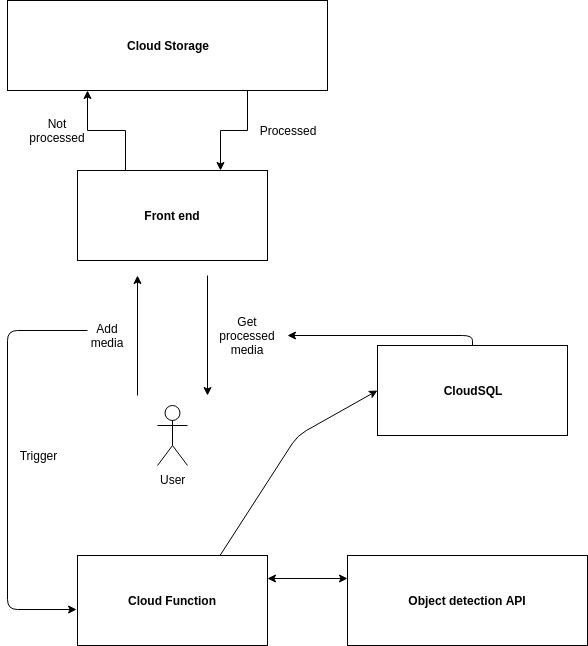
\includegraphics[scale = 0.4]{gcp_pipelinev1.png}
	\caption{GCP pipeline version 1}
	\label{fig:pipelinev1}
\end{figure}

In this version, data would be stored in Google Cloud Storage, the front end would be hosted on a Google Cloud App Engine using NodeJs programming language.

A Golang-written (for performance) cloud function will be triggered when data have been added, calling the AI Platform's hosted model to process it (see ~\ref{fig:pipelinev1}).

\pagebreak
It is a first nice simple solution in theory, but in practice it encounters few problems
\begin{enumerate}
    \item No queue (if you add 100 images, the cloud function will ask a lot to AI Platform, it should wait the end of each processing through a queue)
    \item On the cloud function side again, Python has way more tools to process images, machine learning ... than Golang which is really focused on server side communication
\end{enumerate}

Regarding the use cases here is how it goes for this version:
\begin{enumerate}
    \item Works and on average shouldn't take more than a few seconds maximum: success
    \item The first images will be processed effectively, then a lot of errors and crashes will occurs, overloading the model: fail
    \item All images will have to be uploaded again: fail
    \item This version doesn't handle videos: fail
    \item Everything will crash, no estimations: fail
    \item This version doesn't handle videos: fail
    \item This version doesn't handle videos: fail
    \item This version doesn't handle videos: fail
\end{enumerate}

\pagebreak\subsection{Pipeline version 2}
\begin{figure}[H]
    \centering 
    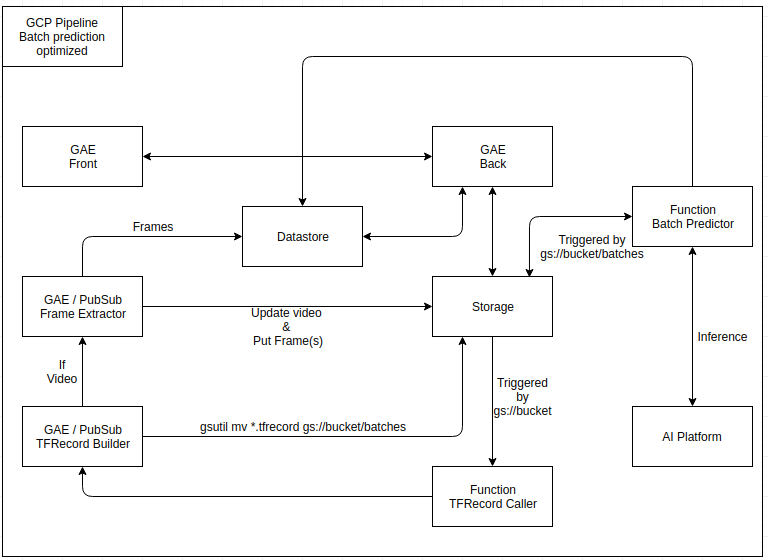
\includegraphics[scale = 0.5]{gcp_pipeline2.png}
	\caption{GCP pipeline version 2}
	\label{fig:pipelinev2}
\end{figure}

The major change here is the use of batch prediction which takes a different kind of input.
Online prediction usually either require an input four dimensions vector of the shape (-1, -1, -1, 3) (first dimension is the number of images, so in online it is always 1, second dimension is the width, third the height and lastly the channel).

Example of 4-d vector input in Python, converting a Numpy array into a serializable list
\begin{lstlisting}[language=Python]
{"inputs": img.tolist()}
\end{lstlisting}

Either it can accept a byte string of the shape (-1), encoded for example in Python:
\begin{lstlisting}[language=Python]
{"inputs": base64.b64encode(jpeg_data)}
\end{lstlisting}

\pagebreak
Batch prediction require the sames types of inputs but stored in a file put in Google Cloud Storage, the file has either a JSON format, a TFRecord format which is the archive format of Tensorflow or a TFRecord GZipped.

TFRecord is way lighter than JSON so an implementation of a TFRecord builder has been developed and deployed in an App Engine.

The second advantage of this version over the first is the introduction of queues through Google Cloud PubSub which handle the communications between Google Cloud services, making concurrent-running components less likely to crash.
This version also includes some more little cloud functions and is more modular (see Figure ~\ref{fig:pipelinev2}).

The problem in this version is the disappearing of online predictions which can be useful for fast predictions, also too many App Engine are used while simple cloud functions would have been enough.

Regarding the use cases here is how it goes for this version:
\begin{enumerate}
    \item This version doesn't handle online prediction: fail
    \item Works and on average shouldn't take more than a few minutes maximum: success
    \item All images will have to be uploaded again: fail
    \item This version doesn't handle online prediction: fail
    \item Possible but no estimations: success
    \item Possible but no estimations: success
    \item Possible, depending in the amount of scaling required: success
    \item Possible, depending in the amount of scaling required but no estimations: success
\end{enumerate}
\pagebreak\subsection{Pipeline version 3}
\begin{figure}[H]
    \centering
    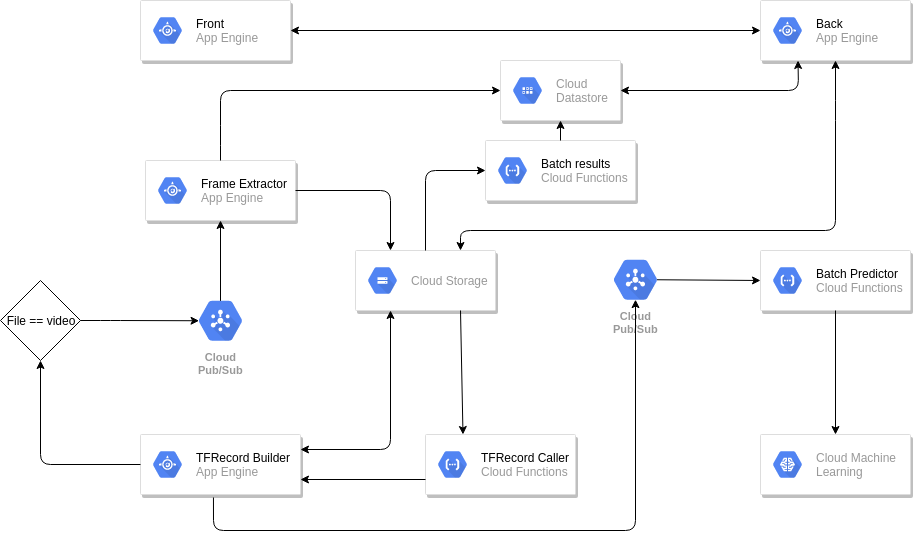
\includegraphics[scale = 0.4]{gcp_pipelinev3.png}
	\caption{GCP pipeline version 3}
	\label{fig:pipelinev3}
\end{figure}

The third version is quite similar to the previous one, some simplifications have been done (see Figure ~\ref{fig:pipelinev3}).

It still lacks online predictions and overuse Google App Engine which are quite expensive.

Regarding the use cases here is how it goes for this version:
\begin{enumerate}
    \item This version doesn't handle online prediction: fail
    \item Works and on average shouldn't take more than a few minutes maximum: success
    \item All images will have to be uploaded again: fail
    \item This version doesn't handle online prediction: fail
    \item Possible but no estimations: success
    \item Possible but no estimations: success
    \item Possible, depending in the amount of scaling required: success
    \item Possible, depending in the amount of scaling required but no estimations: success
\end{enumerate}

\pagebreak\subsection{Pipeline version 4}
\begin{figure}[H]
    \centering
    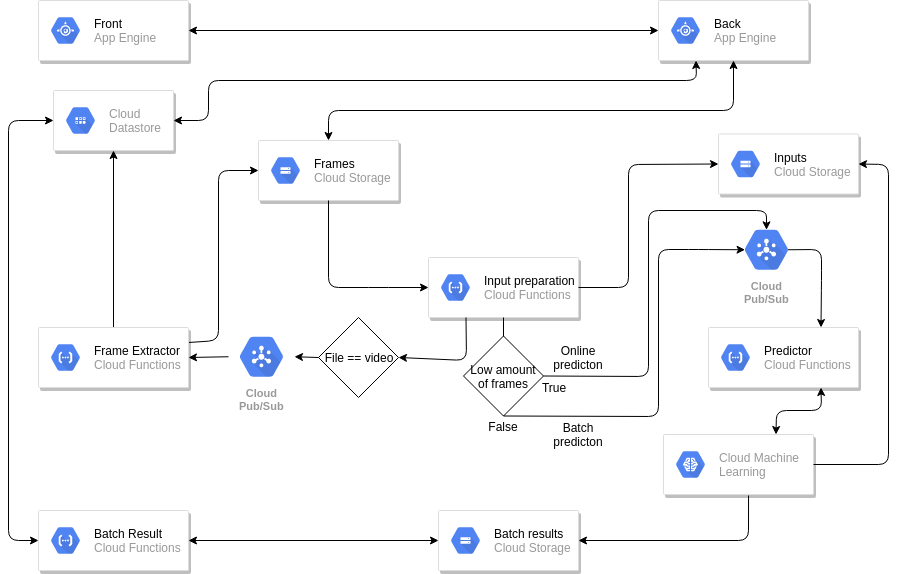
\includegraphics[scale = 0.5]{gcp_pipelinev4.png}
	\caption{GCP pipeline v4}
	\label{fig:pipelinev4}
\end{figure}

The fourth version have evolved through his predecessor, fixing bottlenecks, improving the overall pipeline, handling both batch and online predictions (see Figure ~\ref{fig:pipelinev4}).

The choice between online and batch prediction is customizable by the user, by default batch prediction are preferred over a certain threshold of data to process, under this threshold online predictions are called for fast predictions.

\pagebreak
Regarding the use cases here is how it goes for this version:
\begin{enumerate}
    \item Works and on average shouldn't take more than a few seconds maximum: success
    \item Works and on average shouldn't take more than a few minutes maximum: success
    \item All images will have to be uploaded again: fail
    \item Works and on average shouldn't take more than a few minutes maximum: success
    \item Possible but no estimations: success
    \item Possible but no estimations: success
    \item Possible, depending in the amount of scaling required: success
    \item Possible, depending in the amount of scaling required but no estimations: success
\end{enumerate}

In the end, the only lacking features are price and time estimations before and after upload and the change of model, both are easy to implement and shouldn't take more than a few hours, the biggest part of the architecture was the front end, back end and make everything communicate well together, in addition of the fact AI Platform batch jobs require 6 minutes to boot at cold start, so it took a while to test everything.

\pagebreak\subsection{Components}

Now all components of this final pipeline will be described in detail.

\textbf{Front} component is in charge of directly interfacing with user, it allows to upload images and videos, get prediction results, see statistical graphics about the occurrences of animals over time and space.
It communicates with \textbf{Back} to send images, retrieve predictions and statistics.
\textbf{Front} is implemented with Lit-Element as a single page application.

\textbf{Back} is a REST API implemented in JavaScript with Express package, it saves information about frames and predictions in \textbf{Cloud Datastore}. It stores images and videos in \textbf{Cloud Storage}.
It runs on App Engine so it can scales to any number of instances to handle higher traffic.

\textbf{Cloud Datastore} is a NoSQL database which stores frames, videos, predictions and detected objects, it is convenient to be able to iterate fast without having to define the schema of the database first.

\textbf{Cloud Storage} is a scalable filesystem to store large amount of files, it is used to store images, videos, batch predictions inputs and outputs.

\textbf{Frame extractor} is a cloud function that split videos into frames and store them in \textbf{Cloud Storage} and their metadata in \textbf{Cloud Datastore}.

\textbf{Input preparation} is responsible for building the input of both online and batch predictions from frames and storing it on \textbf{Cloud Storage}. It retrieves the frames from \textbf{Cloud Storage} and publish on \textbf{Cloud PubSub} queue.
It chooses between online or batch prediction based on different parameters to fulfill user needs, for example if the user has only few images to tag it makes sense to use online prediction, if he has ten thousands of videos it makes more sense to use batch prediction.

\textbf{Cloud PubSub} is used to limit the calling rate of batch and online prediction. It is useful because Google API are rate-limited to avoid waste of resource. 

\textbf{Batch prediction AI Platform} receive batch of frames and start a job which automatically scales in many workers and output the predictions efficiently for large number of frames, launching a job takes several minutes so it is not used for few frames.
Results are stored in \textbf{Cloud Storage}.

\textbf{Online prediction AI Platform} produces prediction for one frame with low latency, the result is available in the HTTP answer.

\textbf{Batch result} is a cloud function that update the predictions once they are done into \textbf{Cloud Datastore}.

\pagebreak\section{Data flows, number of operations : price \& time estimations}

In the last few years, people are still hesitating to dive in cloud providers like Amazon, Google, Microsoft with the fear of multiple concerns: losing control, security, data protection, performance and price.
The cloud services are usually difficult to estimate in price, here an example use case showing the consumption of storage and cloud operations using this solution in production is described.
The cost in term of storage, Datastore, ... is detailed in next parts

\subsection{Data \& Ops}
A typical use case would be: 
\begin{enumerate}
    \item Reach main page
    \item Upload a picture
    \item Back on main page to see the results (after a while of course)
\end{enumerate}

\subsubsection{Storage}
\begin{itemize}
    \item Two megabytes image
    \item One operation to store the image
\end{itemize}
\subsubsection{Datastore}
\begin{itemize}
    \item Storage of the annotation mapping approximately <= 1000 rows
    \item Two rows Frame entity (store, then update when prediction are ready)
    \item Predictions into Prediction entity 1 row
    \item Objects detected into Object entity < 50 rows (being large)
    \item One operation put class mapping
    \item One operation put frame
    \item One operation prediction
    \item One operation put objects
\end{itemize}
\subsubsection{Function}
\begin{itemize}
    \item One operation input preparation
    \item One operation prediction
\end{itemize}
\subsubsection{PubSub}
\begin{itemize}
    \item One message being stored and published
\end{itemize}
\subsubsection{App Engine}
\begin{itemize}
    \item Two operations frontend rendering main page
    \item One operation front render upload page
    \item One operation back call frames list
    \item One operation back call frames upload
\end{itemize}
\subsubsection{AI Platform}
\begin{itemize}
    \item One operation online prediction
\end{itemize}

\pagebreak\subsection{Price \& Time}
%https://cloud.google.com/products/calculator/#id=8c3bc8ef-79f9-45da-a7f4-eec8337c3cb5

\begin{figure}[H]
    \centering
    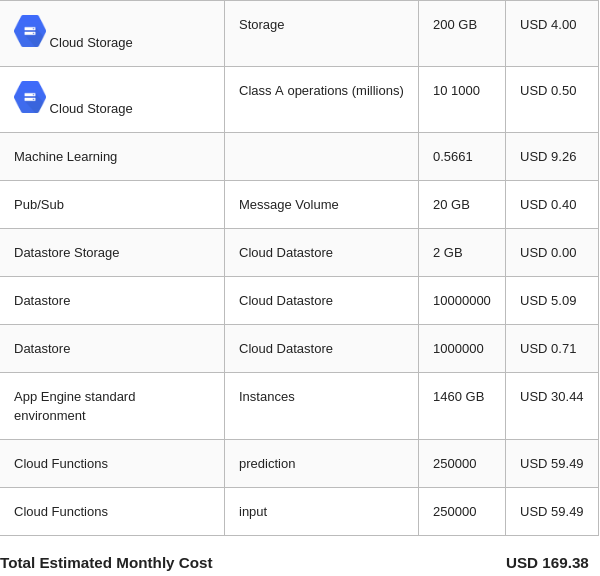
\includegraphics[scale = 0.65]{price_estimation.png}
	\caption{Example price estimation. \href{https://cloud.google.com/products/calculator/\#id=8c3bc8ef-79f9-45da-a7f4-eec8337c3cb5}{Source}}
	\label{fig:priceestimation}
\end{figure}

You can see on Figure ~\ref{fig:priceestimation} the largely estimated price for 100 000 images per month.

This price can probably be highly lowered since no optimization has been done and the "default" and even non needed higher configurations of services have been chosen (2 permanently running App Engine instances, high memory capacity for cloud functions ...).

In addition, creating this estimation helped to recognize where the solution can be optimized to reduce the overall cost.

\pagebreak\section{Statistics}

Statistics based on graphs and other visualizations are available to monitor the evolution of species and their behaviour, some interesting information are:
\begin{itemize}
    \item Occurrence of species over time and zone (plots, charts, histograms, heatmap ...)
    \item Co-occurrence of species, showing the link between them
\end{itemize}

Once a certain amount of data has been generated, one can even imagine using predictive models, from simple linear regression, random forests, boosted trees to neural networks for prevention.

Algorithms to detecting anomalies such as principal component analysis could also help analysing the changes and alert ecologists, for example if a species is suddenly in a sharp decline, this could potentially be the cause of poaching.

Another example would be the strong growth of an invasive mosquito species that would be automatically detected by such algorithms above a certain threshold and would prevent the competent authorities


\pagebreak\section{Used models}

Here a choice needed to be made to take the best model in term of speed / accuracy (mAP) tradeoff AND less than 250mb model to respect AI Platform constraint.

\begin{figure}[H]
    \centering
    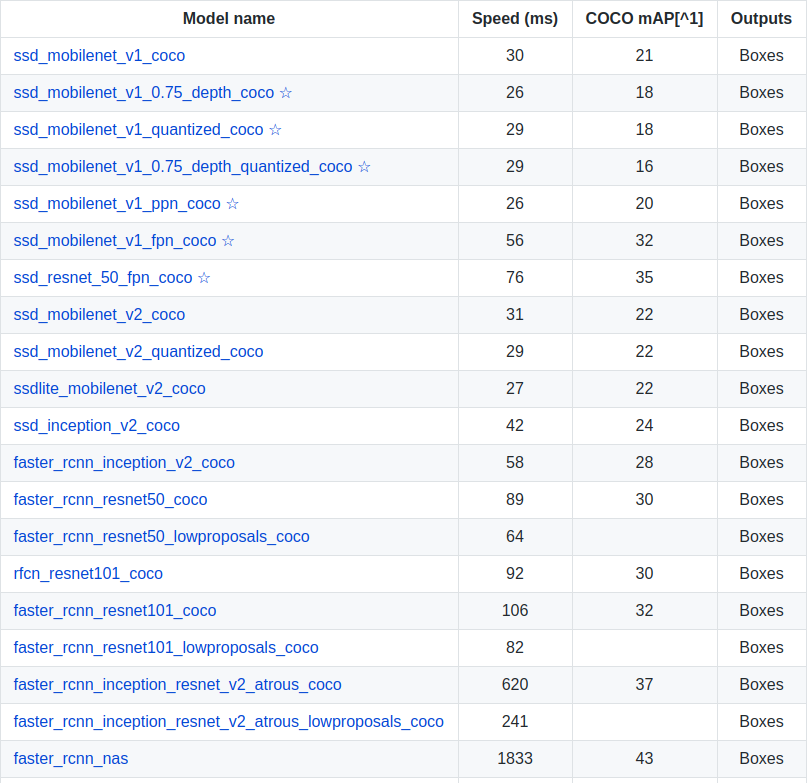
\includegraphics[scale = 0.5]{tensorflow_models_coco_models.png}
	\caption{COCO trained models, speed / accuracy tradeoff. \href{https://github.com/tensorflow/models/blob/master/research/object_detection/g3doc/detection_model_zoo.md}{Source}}
	\label{fig:tfmodels}
\end{figure}

Another constraint was the fact that changing the graph makes the file size grow.

Faster RCNN NAS is the most accurate model obviously because of its neural architecture search algorithm, but 1833 is very high compared to others (see Figure ~\ref{fig:tfmodels}).
An interesting one was SSD ResNet 50 FPN, ending around 180mb after the graph modification.

\pagebreak\section{Performances}

With AI Platform configured with 72 max workers, 1 CPU core and a SSD ResNet50 FPN model, it takes about 20 minutes to process a batch of 10 000 images with a resolution of 100x100 (see Figure ~\ref{fig:10kjob})

\begin{figure}[H]
    \centering
    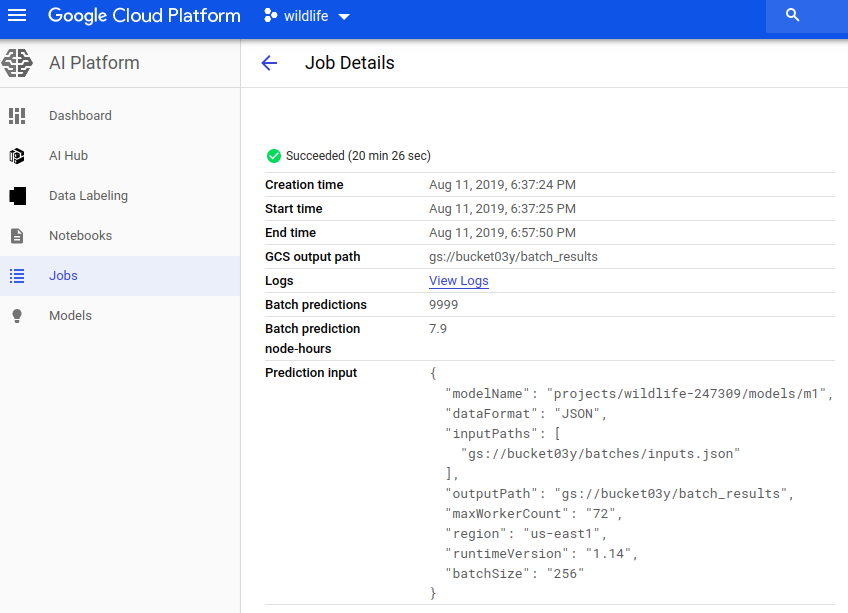
\includegraphics[scale = 2]{10k_job.png}
	\caption{Batch prediction job of 10 000 images}
	\label{fig:10kjob}
\end{figure}

On 	~\ref{fig:10kjob} you can see that in this context it has cost 7.9 node hours at the price of \$0.0791\footnote{see https://cloud.google.com/ml-engine/docs/pricing} which makes a total price of about \$0.6.

\pagebreak\section{Optimization}
In the world of machine learning, the optimization of training is receiving a lot of attention. There is much less information available on inference optimization. 

Yet, isn't serving prediction models the point of ML ?

Serving performance can have a significant impact on the ML value for your use case. Indeed, the cost of inference can be a major factor in the total return on investment of an ML application.

\subsection{Latency (and size) count}
When it comes to optimizing production models, we are mainly concerned with three things:
\begin{itemize}
    \item Model size
    \item Prediction speed
    \item Prediction rate
\end{itemize}

When serving ML, the size of the model is important. Of course, smaller models use less memory, less storage and network bandwidth, and they load faster. In some cases, hardware memory constraints or service limitations may impose a limit on the size of the model. For example, the Machine Learning Engine service on Google Cloud (GCP AI Platform) sets a default size limit of 250 MB for models. 

When we use hardware acceleration for prediction purposes, we must ensure that our model fits into the memory of the acceleration device. The size of the model has a particular impact in situations where we serve it on a peripheral or mobile device with limited capacity. We want the model to be downloaded as quickly as possible, using as little network bandwidth as possible and using as little memory and storage capacity as possible.

Prediction speed is another metric that is important. When we make our online inference, we generally want the results to be returned as quickly as possible. In many online applications, latency is critical to the user experience and application requirements. But we care about the speed of inference, even when we process our data in batches. The inference speed is directly related to the cost of the service, as it is directly related to the amount of computing resources required to make a prediction. The time required to make a prediction will always be a critical variable in any formula that measures the rate of prediction. 

Faster forecasts mean more prediction throughput on the same hardware, resulting in lower costs.
The prediction rate is a measure of the number of predictions that our system can make in a given time period. In addition to the prediction speed mentioned above, other system attributes are involved in determining throughput, including batch processing of forecasts, hardware acceleration, load balancing and horizontal scaling of service instances.


\subsection{Exported model formats in TensorFlow}
TensorFlow has several model serialization formats, but the most important ones to know are the GraphDef and SavedModel formats. 
\begin{itemize}
    \item The GraphDef format is a version of the ProtoBuf\cite{protobuf} serialization protocol, in text or binary form, that codes the definition of a TensorFlow graph. A GraphDef can also include the weights of a trained model, but it does not have to - the weights can be stored in separate control point files. 
    \item The SavedModel format combines a GraphDef with control point files that store weights, all gathered in a folder.
\end{itemize}


\subsection{Tools and techniques}
TensorFlow offers several techniques to reduce the size of a model and improve prediction latency.
Here are some of them:

\begin{itemize}
    \item Freeze: Convert variables stored in a SavedModel control point file to constants stored directly in the model graph. This reduces the overall size of the model.
    \item Pruning: Remove unused nodes in the prediction path and graph outputs, merging duplicate nodes and cleaning other node operations such as summary, identity, etc.
    \item Constant folding: Substitute the values of known constants in expressions at compile time in the sub-graphs of the model
    \item Batch standard folding: Fold the multiplications introduced in the batch normalization into the weight multiplications of the previous layer.
    \item Quantization: Convert floating point weights to lower accuracy, such as 16 or 8 bits.
\end{itemize}

For mobile deployment, there is also TFLite, which performs 8-bit quantification on mobile models.

TensorFlow offer a graph transformation tool to perform most optimizations, which is a C++ command line tool.

The Graph Transform tool is designed to work on models saved as GraphDef files in protobuf format. However, the SavedModel format is the most modern and most supported by other tools and services. This is the only format supported by Google Cloud AI Platform for prediction.
The optimization steps, as well as the model format transitions, are as follows:
\begin{enumerate}
    \item Freeze the exported model: SavedModel => GraphDef
    \item Optimize the fixed model: GraphDef => GraphDef
    \item Convert the optimized frozen model back: GraphDef => SavedModel
\end{enumerate}


\pagebreak\section{Other tools built}
All the tools are publicly available on the main Github repository.

\subsection{Inference graph modification}
Batch prediction on AI Platform cause a problem, when the prediction are done and written to a file, nothing give any information about which prediction is linked to which input.

To solve this problem, a tool to change the graph of the model needed to be developed.

Tensorflow offer a repository specific to models\cite{tensorflow_models}, many tools are available there to work with object detection graphs.
Tensorflow also make the possibility to display a graph through a command-line script.


\begin{figure}[H]
  \centering
  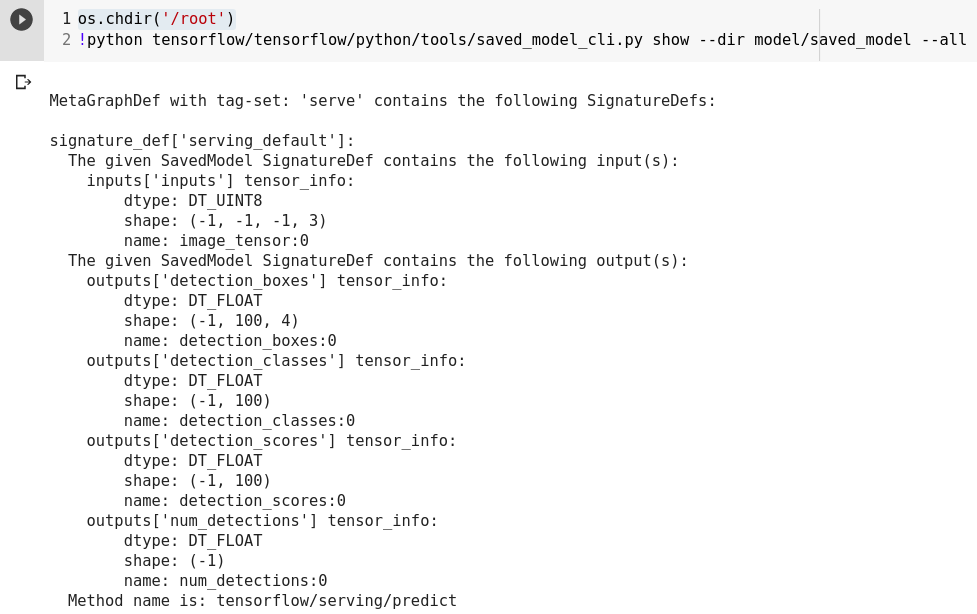
\includegraphics[width=1\linewidth]{initial_graph.png}
  \caption{Initial object detection graph}
  \label{fig:initialgraph}
\end{figure}

A Tensorflow object detection model's graph input and output is shown on Figure ~\ref{fig:initialgraph}.

\begin{figure}[H]
  \centering
  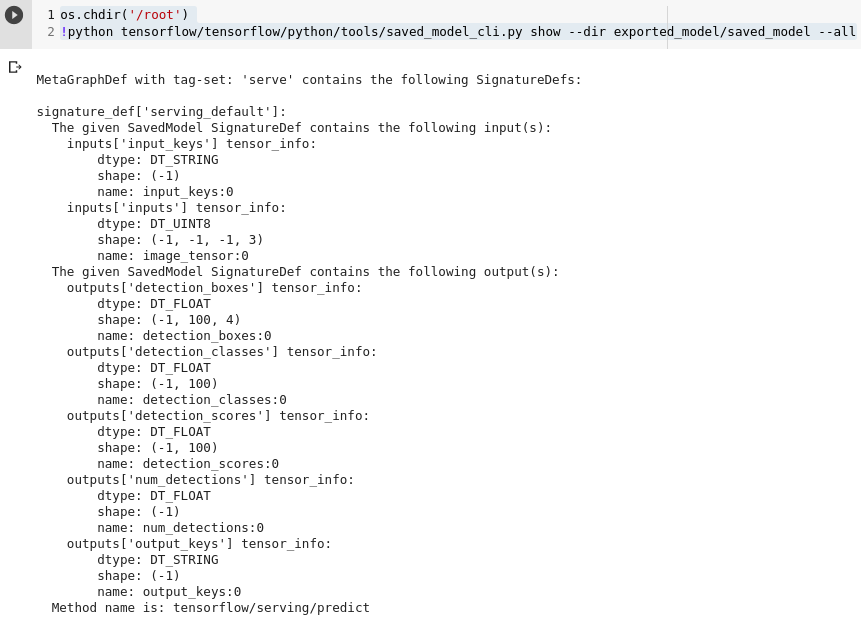
\includegraphics[width=1\linewidth]{modified_graph.png}
  \caption{Changed graph to handle keys}
  \label{fig:changedgraph}
\end{figure}

Then you can see on Figure ~\ref{fig:changedgraph} the modified graph with the input and output keys used to map an image to its prediction (E.g. I detected a cat at top-left ...)

A fork and modification of Tensorflow Models repository has been done\footnote{See https://github.com/louis030195/models} to allow such graph modification.

\subsection{Gitpod configurations}

The growth of cloud services made also available cloud development possible, an example of this is Google Colaboratory\cite{colab} which have been of great use but is only for Python, Gitpod\cite{gitpod} allows to develop in most languages.

A customised Docker configuration has been developed to allow ready-to-code environment in a click\footnote{see https://github.com/louis030195/vision-client}.
